\section{Articulated Rigid Body Dynamics}
We now derive the equations of motion for an articulated rigid body structure. We follow the derivation of rigid body dynamics in generalized coordinates from \secref{rigidbodydyngen}.

An articulated rigid body system is represented as a set of rigid bodies connected through joints in a tree structure. Every rigid link has exactly one \emph{parent} joint. The joint corresponding to the root of the tree is special since it does not link the root to any other rigid link. The generalized coordinates are the DOFs of the root link of the tree (that may represent the global translation and rotation), and the joint angles corresponding to the admissible joint rotations for all the other joints. 

\subsection{Definitions}
The state of an articulated rigid body
system can be expressed as $(\vc{x}_k, R_k, \vc{v}_k,
\boldsymbol{\bm{\omega}}_k)$, where $k = 1, \cdots, m$ and $m$ is the number of rigid links. Here $\vc{x}_k$ and
$R_k$ are the position of the COM and the orientation of the rigid link $k$, and $(\vc{v}_k,
{\bm{\omega}}_k)$ are the linear and angular velocity of the
rigid link $k$ viewed in the world frame. Similarly, we define the
Cartesian force and torque applied on rigid link $k$ as $(\vc{f}_k,
{\bm{\tau}}_k)$, both of which are expressed in the world
frame.

The same articulated rigid body system can be represented in
generalized coordinates. We define the generalized state as $(\vc{q},\dot{\vc{q}})$, where $\vc{q} = (\vc{q}_1,\hdots,\vc{q}_k,\hdots,\vc{q}_m)$ and each $\vc{q}_k$ is the set of DOFs of the joint that connects the link $k$ to its parent link (see \figref{example1}). 

\begin{wrapfigure}{r}{0.4\textwidth}
 \vspace{20pt}
\begin{center}
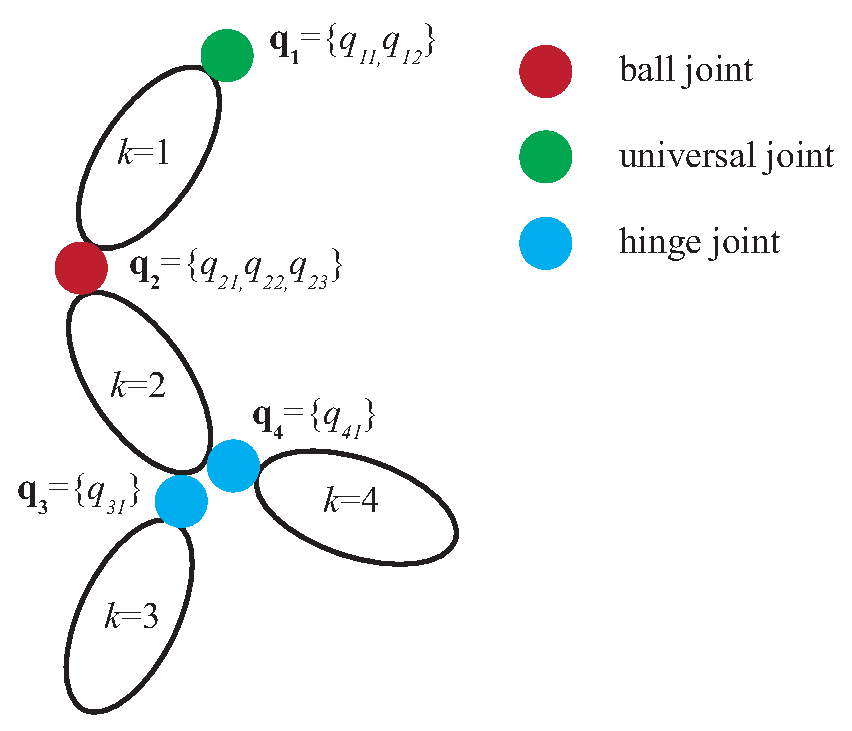
\includegraphics[width=2.1in]{example1_new.eps}
\end{center}
\caption{An articulated system.}
 \vspace{0pt}
\label{fig:example1}
\end{wrapfigure}

We list a few notations and definitions for an articulated rigid body system with $m$ rigid links. 
\begin{itemize}
\item $p(k)$ returns the index of the parent link of link $k$. For
  example in Figure \ref{fig:example1}, $p(4) = 2$. $p(1,k)$ returns the indices of all the links in the chain from the root to the link $k$ (including $k$). For example, $p(1,4) = \{1,2,4\}$
\item $n(k)$ returns the number of DOFs in the joint that connects the $k$ to the parent link $p(k)$. For example in Figure \ref{fig:example1}, $n(2) = 3$, $n(3) = 1$ etc. We denote the total number of DOFs in the system by $n$. \eg $n=7$ in Figure \ref{fig:example1}.
\item $R_k$ is the local rotation matrix for the link $k$ and depends only on the DOFs $\vc{q}_k$. $R^0_k$ is the chain of rotational transformations from the
  world frame to the local frame of the link $k$. Therefore, $R^0_k = R^0_{p(k)}R_k$. Since the link $1$ does not have a parent link, $R^0_{p(1)} = \vc{I}_3$.
\end{itemize}



\subsection{Cartesian and generalized velocities}

For a single rigid body, \eqnref{vellin} and \eqnref{velang} describe the relation between the Cartesian velocities and the generalized velocities. 
For an articulated rigid body system, we use the same recipe as rigid body dynamics in \secref{rigidbodydyngen} and define the Jacobians for each rigid link that relate its respective Cartesian velocities to the generalized velocity of the entire system. 

We start with deriving the relation for the angular velocity. The angular velocity of link $k$ viewed in the world frame is:
\begin{eqnarray}
\nonumber
[\bm{\omega}_k] & = & \dot{R}^0_k {R^0_k}^T = \dot{(R^0_{p(k)}R_k)} (R^0_{p(k)}R_k)^T\\
\nonumber
& = & (\dot{R}^0_{p(k)}R_k + {R^0_{p(k)}}\dot{R}_k)  R_k^T {R^0_{p(k)}}^T \\
\label{eq:angvelk_recursive}
& = & \dot{R}^0_{p(k)}{R^0_{p(k)}}^T + R^0_{p(k)} \left ( \dot{R}_k R_k^T \right ) {R^0_{p(k)}}^T \equiv [\bm{\omega}_{p(k)}] + R^0_{p(k)} [\hat{\bm{\omega}}_k] {R^0_{p(k)}}^T
%& = & [\bm{\omega}_{p(k)}] +  [R^0_{p(k)} \hat{\bm{\omega}}_k] = [\bm{\omega}_{p(k)} + R^0_{p(k)} \hat{\bm{\omega}}_k]
\end{eqnarray}
In the above equation, we define [$\hat{\bm{\omega}}_k] = \dot{R_k} R_k^T$ that denotes the angular velocity of the link $k$ in the frame of its parent link $p(k)$ since the rotation matrix $R_k$ is the rotation of the rigid link $k$ with respect to $p(k)$. We can further write $\hat{\bm{\omega}}_k = \hat{J}_{\omega k} \dot{\vc{q}}_k$ where $\hat{J}_{\omega k}$ is the \emph{local} Jacobian matrix that relates the joint velocity of link $k$ to its angular velocity in the frame of the parent link $p(k)$. The dimension of $\hat{J}_{\omega k}$ is $3\times n(k)$. 

Using the property of skew symmetric matrix, $[R \bm{\omega}] = R [\bm{\omega}]
R^T$, we can express \eqnref{angvelk_recursive} in the vector form as:
\begin{eqnarray}
\label{eq:angvelk_iterative}
\nonumber
\bm{\omega}_k & = & \bm{\omega}_{p(k)} + R^0_{p(k)} \hat{J}_{\omega k} \dot{\vc{q}}_k\\
\nonumber
& = & \sum_{l \in p(1,k)} R^0_{p(l)} \hat{J}_{\omega l} \dot{\vc{q}}_l \mbox{\ \ (By unrolling the recursive definition)}\\
& \equiv & J_{\omega k}\dot{\vc{q}}
\end{eqnarray}
where the Jacobian $J_{\omega k}$ is:
\begin{equation}
\label{eq:angular_velocity_jac_link}
J_{\omega k} = \left ( \hat{J}_{\omega 1}\;\; \hdots\;\; R^0_{p(l)} \hat{J}_{\omega l} \;\;\hdots\;\; \vc{0} \;\;\hdots \right )
\end{equation}

Note that the zero matrices \vc{0} of size $3\times n(l)$ in $J_{\omega k}$ correspond to
joint DOFs $\vc{q}_l$ that are \emph{not} in the chain of transformations from the root to the
link $k$. 
Let us look at a couple of examples using the articulated
rigid body system in Figure \ref{fig:example1}:
\begin{eqnarray}
\bm{\omega}_1 &=& (\hat{J}_{\omega 1} \;\; \vc{0}
\;\;\vc{0}\;\;\vc{0}) \dot{\vc{q}}  \nonumber \\
\bm{\omega}_4 &=& (\hat{J}_{\omega 1} \;\; R^0_1\hat{J}_{\omega 2} \;\;
\vc{0} \;\;
R^0_2 \hat{J}_{\omega 4}) \dot{\vc{q}} \nonumber
\end{eqnarray}
where $\hat{J}_{\omega 1} \in \Re^{3\times2}$, $\hat{J}_{\omega 2} \in \Re^{3\times3}$ and $\hat{J}_{\omega 4} \in \Re^{3\times1}$.
Depending on the representation of the rotation $\vc{q}_k$,
$\hat{J}_{\omega k}$ can assume different values and dimensions. For example, if the joint
between link $1$ and link $2$ in Figure \ref{fig:example1} is
represented as three Euler rotations, $R^{(x)}$, $R^{(y)}$, and
$R^{(z)}$ such that $R_2(\vc{q}_2)= R^{(x)}(q_{21}) R^{(y)}(q_{22}) R^{(z)}(q_{23})$, we have:
\begin{equation}
\hat{J}_{\omega 2} = 
\begin{pmatrix}
\begin{array}{c}
1\\
0\\
0
\end{array}
&
R^{(x)} \Bigg (
\begin{array}{c}
0\\
1\\
0
\end{array} 
\Bigg )
&
R^{(x)} R^{(y)}\Bigg (
\begin{array}{c}
0\\
0\\
1
\end{array} 
\Bigg )
\end{pmatrix}
\end{equation}
If the joint is represented as a quaternion or an
exponential map, $\hat{J}_{\omega k}$ does not have a simple form. As an example, the relation between the rotation matrix $R_k$ and the exponential map representation $\vc{q}_k=(q_{k1},q_{k2},q_{k3})$ can be written as:
\begin{equation}
R_k(\vc{q}_k) = e^{[\vc{q}_k]} = \vc{I}_3 + \frac{sin \theta}{\theta} [{\vc{q}}_k] + \frac{1-cos \theta}{\theta^2}[{\vc{q}}_k]^2
\end{equation}
where $\theta = ||\vc{q}_k ||$. The Jacobian $\hat{J}_{\omega k}$ can be derived by equating the result of $\dot{R}_k R_k^T$ to $[\hat{J}_{\omega k} \dot{\vc{q}}_k]$:
\begin{eqnarray}
\nonumber
\hat{J}_{\omega k} & = & R_k \left ( \vc{I}_3 - \frac{1-cos\theta}{\theta^2}[\vc{q}_k] + \frac{\theta - sin \theta}{\theta^3} [\vc{q}_k]^2 \right )\\
 & = & \vc{I}_3 + \frac{1-cos\theta}{\theta^2}[\vc{q}_k] + \frac{\theta - sin \theta}{\theta^3} [\vc{q}_k]^2
\end{eqnarray}
For the case when $\theta \rightarrow 0$, $R_k$ and $\hat{J}_{\omega k}$ can be approximated as follows:
\begin{eqnarray}
R_k & = & \vc{I}_3 + [{\vc{q}}_k] + \frac{1}{2}[{\vc{q}}_k]^2\\
\hat{J}_{\omega k} & = & \vc{I}_3 + \frac{1}{2}[{\vc{q}}_k] + \frac{1}{6}[{\vc{q}}_k]^2
\end{eqnarray}
\ignorethis{
\begin{equation}
\label{eq:angular_velocity_link}
\bm{\omega}_k = (\vc{s}_1 \cdots \vc{s}_{np} \; R^0_{k-1} \vc{t}_1 \cdots
R^0_{k-1} \vc{t}_{nk}\; \vc{0} \cdots \vc{0}) \dot{\vc{q}} = J_{\omega k} \dot{\vc{q}}
\end{equation}
where $np$ is the number of DOFs in the parent chain and $nk$ is the
number of DOFs in the link $k$. 
}
Similar to the angular velocity, the linear velocity of the center of mass of the link $k$
can be expressed in terms of the generalized velocity: 
\begin{equation}
\label{eq:linear_velocity_link}
\vc{v}_k = J_{vk} \dot{\vc{q}}, \;\;\;\mathrm{where}\;\; J_{vk} = \frac{\partial \vc{x}_k}{\partial \vc{q}}=  \frac{\partial W^0_k
  \vc{c}_k}{\partial \vc{q}}.
\end{equation}
where the chain of homogeneous transformations from the world frame to the local
frame of link $k$ is denoted as $W^0_k$. Note that $W^0_k$ is
different from $R^0_k$ in that $W^0_k$ includes the translational
transformations. $\vc{c}_k$ is a constant vector that denotes the center of mass of link $k$ in
its local frame.

We can concatenate the Cartesian velocities into a single vector $\vc{V}_k$ and denote the relation as:
\begin{eqnarray}
\label{eq:vel_relation_link}
\nonumber
\vc{V}_k & = & {J}_k \dot{\vc{q}}\\
\mbox{where } & & 
\vc{V}_k = \left (
\begin{array}{c}
\vc{v}_k\\
\bm{\omega}_k
\end{array}
\right ) \mbox{and\ }
{J}_k = \left (
\begin{array}{c}
J_{vk}\\
J_{\omega k}
\end{array}
\right ) 
\end{eqnarray}


\subsection{Equations of motion}
We now derive the equations of motion of an articulated rigid body system in generalized coordinates. The kinetic energy $T$ of the entire system can be expressed as the sum of kinetic energies of all the rigid links as $T=\sum_k T_k$. Therefore the equations of motion of the system can be computed as:
\begin{eqnarray}
\nonumber
\frac{d}{dt} \left ( \frac{\partial T}{\partial \dot{\vc{q}}} \right ) - \frac{\partial T}{\partial \vc{q}} & = & \frac{d}{dt} \left ( \frac{\partial \sum_k T_k}{\partial \dot{\vc{q}}} \right ) - \frac{\partial \sum_k T_k}{\partial \vc{q}}\\
\nonumber
& = & \sum_k \left ( \frac{d}{dt} \left ( \frac{\partial T_k}{\partial \dot{\vc{q}}} \right ) - \frac{\partial T_k}{\partial \vc{q}} \right )\\
\nonumber
& = & \sum_k \left ( \left( J_k^T M_{ck} J_k \right )\ddot{\vc{q}} + \left( J_k^T M_{ck} \dot{J}_k + J_k^T [\tilde{\bm{\omega}}_k]M_{ck} J_k \right )\dot{\vc{q}} \right )\\
& = &  \sum_k \left( J_k^T M_{ck} J_k \right )\ddot{\vc{q}} + \sum_k\left( J_k^T M_{ck} \dot{J}_k + J_k^T [\tilde{\bm{\omega}}_k]M_{ck} J_k \right )\dot{\vc{q}}
\end{eqnarray}
In deriving the above equation, we use the equations of motion in generalized coordinates for a single rigid body defined in \eqnref{dyngen_vec} subscripted by $k$ for the dynamics of $k^{th}$ link in the multibody system. The Jacobian $J_k$ for the $k^{th}$ link is defined in \eqnref{vel_relation_link}.

